%% Complex Numbers
        
        \section{Introduction to Complex Numbers}
        
        Complex numbers are a wonderful part of mathematics.  You, as the reader, have seen them before.  However, there is a lot of power hiding within this number system.  We will start our venture into this course with this topic as it is a set up for a lot to come.  Quantum theory utilizes complex numbers right out of the gate, and we will as well.
        
        There is a whole branch of study devoted to the calculus of complex numbers called \emph{complex analysis}. Maybe you'll find this interesting and wish to take Math 419!  We will not actually dive into the (slightly different) calculus for these numbers, but rather need them as a tool.
        
        You see, we will always need to be able to factor polynomial equations. This is the biggest benefit to using complex numbers as we will see with the \emph{Fundamental Theorem of Algebra.} We do not prove this theorem, but merely state it. One should always remember fundamental theorems.
        
        Imaginary numbers are those we find by taking the square root of a negative number.  By appending imaginary numbers to the set of real numbers $\R$, we create the complex numbers $\C$. For us, the ability to find a square root of -1 will be powerful. It will help us solve differential equations and do linear algebra.
        
        \begin{question}
        What is a complex number? What was the motivation for developing them?
        \end{question}
        
        \begin{answer}
        Let me begin by answering the second part of the question.\\  
        
        \noindent Take a polynomial,
        \[
        a_0+a_1 z + a_2 z^2 + \cdots + a_n z^n.
        \]
        When does this polynomial equal zero?  In other words, what are the \emph{roots} of this polynomial?
        
        The fact of the matter is that the real numbers $\R$ are just \underline{not} large enough to guarantee that we have all possible roots. Take, for example, the polynomial
        \[
        x^2+1.
        \]
        Set this equal to zero and we have
        \begin{align*}
            x^2+1&=0\\
            \implies x^2&=-1\\
            \implies x&=\pm \sqrt{-1}.
        \end{align*}
        It seems that we are missing a number in this case.  Specifically, 
        \[
        \sqrt{-1}\notin \R.
        \]
        Let us take this new number and denote
        \[
        i\coloneqq\sqrt{-1}.
        \]
        Of course this also means that
        \[
        i^2=-1.
        \]
        A complex number will be made with real numbers and this new additional member. We call $i$ the \boldgreen{imaginary number}\index{imaginary!number}.  It's too bad this number has been named imaginary as it is certainly very physical.
        \end{answer}
        
        \begin{df}{Complex Number; Real and Imaginary Part}{complex_num}
        We can generate any complex number by combining a real number with an imaginary number. Specifically, we can write a \boldgreen{complex number}\index{complex!number} $z$ as
        \[
        z=a+bi
        \]
        where $a,b\in \R$. We call this form $z=a+bi$ the \boldgreen{cartesian}\index{cartesian} or \boldgreen{rectangular form} of a complex number. We also call $a$ the \boldgreen{real part} of $z$ and $b$ the \boldgreen{imaginary part}\index{imaginary!part} of $z$.  We will write
        \[
        \RE(z)=a \qquad \IM(z)=b,
        \]
        and typically let $z$ denote a complex number. Notice that we do \underline{not} include $i$ with the imaginary part!
        \end{df}
        
        \noindent Let us also denote the set of all complex numbers by $\C$ (just as we denoted the real numbers by $\R$). It's important to remember that there is really no way to simplify this number further. There are other ways to specify a complex numbers but they will have real and imaginary parts like this.
        
        The amazing fact about complex numbers is that they allow us to factor (or find the zeros of) \emph{any} polynomial
        \[
        a_0+a_1 z + a_2 z^2 + \cdots + a_{n-1}z^{n-1}+ a_n z^n
        \]
        even when the coefficients $a_i$ are complex themselves.  This fact is known as the \emph{fundamental theorem of algebra}.
        
        \begin{thm}{Fundamental Theorem of Algebra}{FTA}
        Let $f(z)$ be an a polynomial of degree $n$. That is,
        \[
        f(z)=a_0+a_1 z + a_2 z^2 + \cdots + a_{n-1} z^{n-1} + a_n z^n.
        \]
        Then $f(z)$ \emph{always} has $n$ complex roots.
        \end{thm}
        
        \section{Complex Number Algebra}
        
        With a new number system, we must ask how we treat it algebraically. Given two complex numbers $z_1=a_1+b_1i$ and $z_2=a_2+b_2i$ we can write the following:
        \begin{itemize} 
            \item \textbf{Addition:} We add complex numbers by
            \[
            z_1+z_2=(a_1+b_1i)+(a_2+b_2i)=(a_1+a_2)+(b_1+b_2)i.
            \]
            That is to say that we add by adding the real parts together and the imaginary parts together. 
            
            \item \textbf{Multiplication:} We can multiply complex numbers in the same way we multiply polynomials.  In other words, we distribute.  So we have
            \begin{align*}
            z_1\cdot z_2 &= (a_1+b_1i)\cdot (a_2+b_2i)\\
            &= a_1a_2+a_1b_2i+a_2b_1i+b_1b_2(i)^2\\
            &=(a_1a_2-b_1b_2)+(a_1b_2+a_2b_1)i.
            \end{align*}
            Notice that we used the fact that $i^2=-1$.
        \end{itemize}
        
        \begin{exercise}
        What are the real and imaginary parts of the above two examples?
        \end{exercise}
        
        For real numbers $x$ we had that
        \[
        x+(-x)=0.
        \]
        We also could find a number called the inverse of $x$ and denoted by $x^{-1}$ so that
        \[
        x\cdot x^{-1}=1,
        \]
        unless $x=0$. We can mimic these properties with complex numbers as well. Before we do this, let me introduce one concept first that will prove to be very useful. 
        
        \begin{df}{Complex Conjugate}{comp_conj}
        Given a complex number $z=a+bi$ we define the \boldgreen{complex conjugate of $z$}\index{complex!conjugate} (denoted $z^*$) by
        \[
        z^* = a-bi.
        \]
        \end{df}
        
        \begin{itemize}
            \item The negative of a complex number is just the negative of both the real and imaginary part. So if we are given $z=a+bi$ then the negative is $-z=-a-bi$.  We can check that this gives us the desired property by
            \[
            z+(-z)=(a+bi)+(-a-bi)=0.
            \]
            \item To find the inverse of $z=a+bi$ which we call $z^{-1}$, we write $z^{-1}=\frac{1}{a+bi}$.  This way we definitely have
            \[
            z\cdot z^{-1}=\frac{a+bi}{a+bi}=1.
            \]
            However, we haven't written $z^{-1}$ in our standard form! Let us fix this. Take $z=a+bi$ so that $z^{-1}=\frac{1}{a+bi}$.  We can multiply the numerator and denominator by $z^*$ and we find
            \[
            \frac{z^*}{z^*\cdot (a+bi)}=\frac{a-bi}{(a-bi)(a+bi)}=\frac{a-bi}{a^2+b^2}
            \]
            which means that we can write
            \[
            z^{-1}=\frac{a}{a^2+b^2}-\frac{b}{a^2+b^2}i.
            \]
        \end{itemize}
        
        This actually serves to motivate the geometry of complex numbers which we will visit next. As always, having more than one way of understanding a concept helps. One may find that they understand the algebraic or geometric point of view better.  We're unique individuals after all!
        
        \section{Geometry of complex numbers}
        
        With the algebra out of the way, we can concentrate on the geometry of $\C$ for a bit.  The complex numbers turn out to be wonderfully geometrical. We begin with the complex plane $\C$.  The way we usually plot points in $\C$ is by looking at the real and imaginary parts of a complex number $z$.  
        
        \begin{center}
        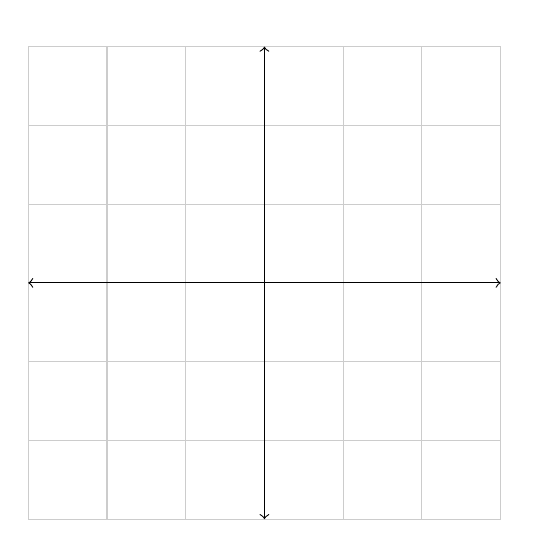
\begin{tikzpicture}
        \draw[thin,gray!40] (-3,-3) grid (3,3);
        \draw[<->] (-3,0)--(3,0) node[right]{$\RE$};
        \draw[<->] (0,-3)--(0,3) node[above]{$\IM$};
        \end{tikzpicture}
        \end{center}
        
        So, for example, let us plot a few points in the complex plane. We'll take
        \[
        z_1=1+i \qquad z_2=-1+i \qquad z_3=2-2i \qquad z_4=-2-i
        \]
        
        \begin{center}
        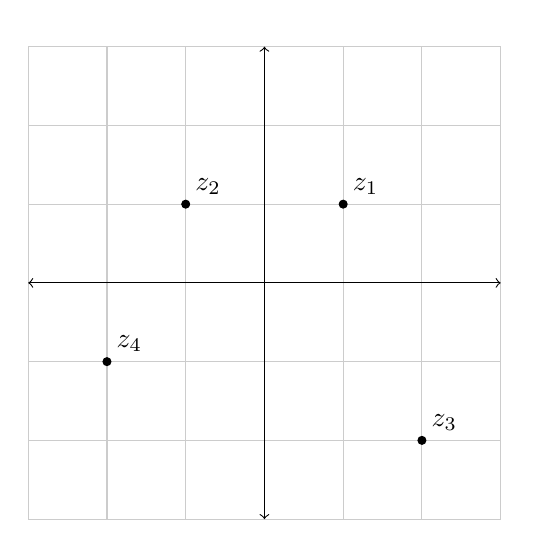
\begin{tikzpicture}
        \draw[thin,gray!40] (-3,-3) grid (3,3);
        \draw[<->] (-3,0)--(3,0) node[right]{$\RE$};
        \draw[<->] (0,-3)--(0,3) node[above]{$\IM$};
       %\addplot+[only marks] coordinates {(1,1) (-1,1) (2,-2) (-2,-1)};
        \foreach \Point/\PointLabel in {(1,1)/z_1, (-1,1)/z_2, (2,-2)/z_3, (-2,-1)/z_4}
        \draw[fill=black] \Point circle (0.05) node[above right] {$\PointLabel$};
        \end{tikzpicture}
        \end{center}
        
        \noindent Let us investigate what our algebra was doing geometrically!\\
        
        \noindent\boldgreen{Addition of complex numbers:} Recall that if we have $z_1=a_1+b_1 i$ and $z_2=a_2+b_2 i$ then
        \[
        z_1+z_2 = a_1+a_2 + (b_1 +b_2)i.
        \]
        With an explicit example, let us take
        \[
        z_1 = 1+i \qquad z_2=1-2i
        \]
        Then
        \[
        z_3=z_1+z_2=2-i.
        \]
        We can plot these in the complex plane like so.
        \begin{center}
        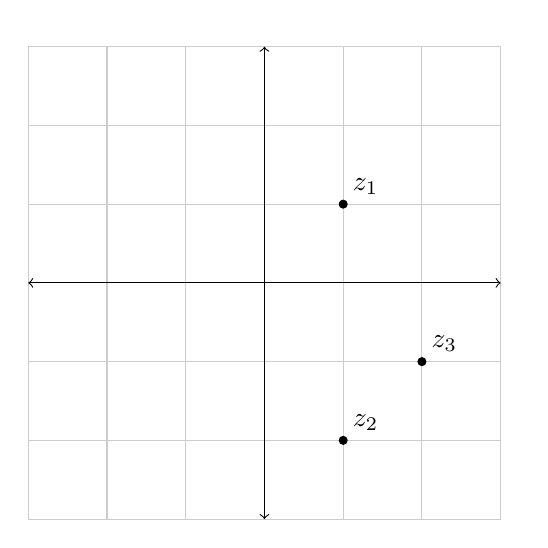
\begin{tikzpicture}
        \draw[thin,gray!40] (-3,-3) grid (3,3);
        \draw[<->] (-3,0)--(3,0) node[right]{$\RE$};
        \draw[<->] (0,-3)--(0,3) node[above]{$\IM$};
       %\addplot+[only marks] coordinates {(1,1) (-1,1) (2,-2) (-2,-1)};
        \foreach \Point/\PointLabel in {(1,1)/z_1, (1,-2)/z_2, (2,-1)/z_3}
        \draw[fill=black] \Point circle (0.05) node[above right] {$\PointLabel$};
        \end{tikzpicture}
        \end{center}   
        The other way of thinking about this addition is to think of attaching arrows to each other.  If we draw an arrow from the \emph{origin} $z=0$ to our desired point $z_i$, we can then use these arrows to perform addition.  If we take a copy of the arrow from the origin to $z_2$ and glue it to the head of the arrow from the origin to $z_1$ we arrive at our point $z_3$.
        \begin{center}
        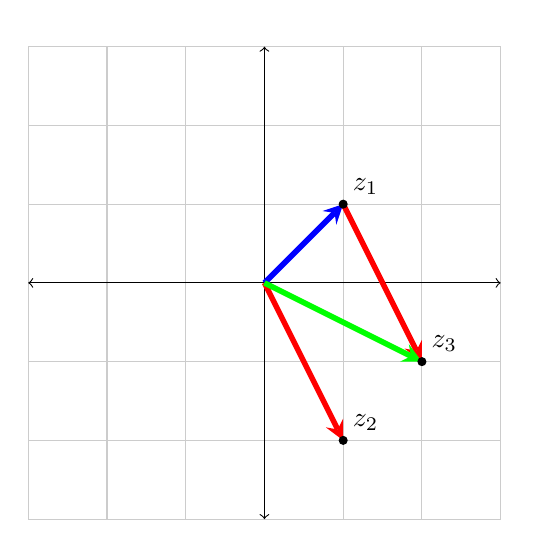
\begin{tikzpicture}
        \draw[thin,gray!40] (-3,-3) grid (3,3);
        \draw[<->] (-3,0)--(3,0) node[right]{$\RE$};
        \draw[<->] (0,-3)--(0,3) node[above]{$\IM$};
        \draw[line width=2pt,blue,-stealth](0,0)--(1,1) node[anchor=east] at (1,1){};
        \draw[line width=2pt,red,-stealth](0,0)--(1,-2) node[anchor=east] at (1,-2){};
        \draw[line width=2pt,red,-stealth](1,1)--(2,-1) node[anchor=east] at (2,-1){};
        \draw[line width=2pt,green,-stealth](0,0)--(2,-1) node[anchor=east] at (2,-1){};
        \foreach \Point/\PointLabel in {(1,1)/z_1, (1,-2)/z_2, (2,-1)/z_3}
        \draw[fill=black] \Point circle (0.05) node[above right] {$\PointLabel$};
        \end{tikzpicture}
        \end{center}
        
        How about the complex conjugate? What was this doing? Given a complex number $z=a+bi$, we know that $z^*=a-bi$.  So, take the example
        \[
        z=2+2i \qquad z^*=2-2i.
        \]
        \begin{center}
        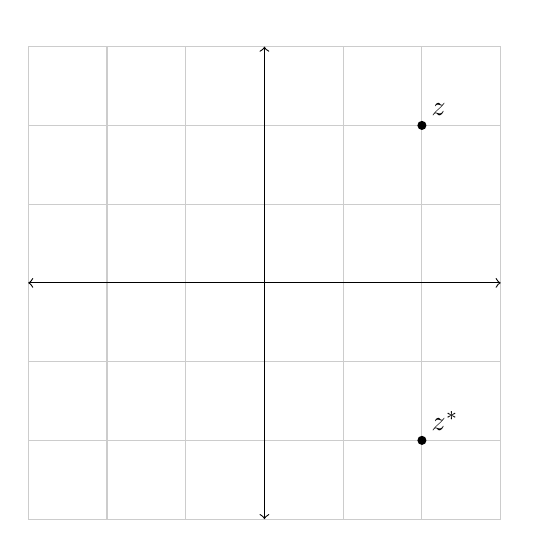
\begin{tikzpicture}
        \draw[thin,gray!40] (-3,-3) grid (3,3);
        \draw[<->] (-3,0)--(3,0) node[right]{$\RE$};
        \draw[<->] (0,-3)--(0,3) node[above]{$\IM$};
       %\addplot+[only marks] coordinates {(1,1) (-1,1) (2,-2) (-2,-1)};
        \foreach \Point/\PointLabel in {(2,2)/z, (2,-2)/z^*}
        \draw[fill=black] \Point circle (0.05) node[above right] {$\PointLabel$};
        \end{tikzpicture}
        \end{center}
        Notice that complex conjugation is just reflection about the real axis!  
        
        \section{Polar coordinates}
        An extremely important notion in planar geometry is that of \emph{polar coordinates}. Usually, we are happy to reference a point in the plane by giving the $x$-coordinates and $y$-coordinates.  In the complex case, we can give the $\RE$ and $\IM$ parts of the complex number to specify its location in the complex plane $\C$.
        
        There are many different ways you could choose to represent points in the plane, but almost all of them are rather silly to a human.  However, one that provides a great bit of intuition is polar coordinates. The idea is as follows:
        
        \begin{df}{Polar Coordinates}{pol_coord_df}
        \boldgreen{Polar coordinates}\index{polar coordinates} are the a coordinate system that uses $r$, the distance from the origin, and $\theta$, the counter-clockwise angle measured from the $\RE$ axis in the complex plane $\C$ (or $x$-axis in $\R^2$).
        \end{df}
        
        The following image may prove to be helpful.  
        
        \begin{center}
  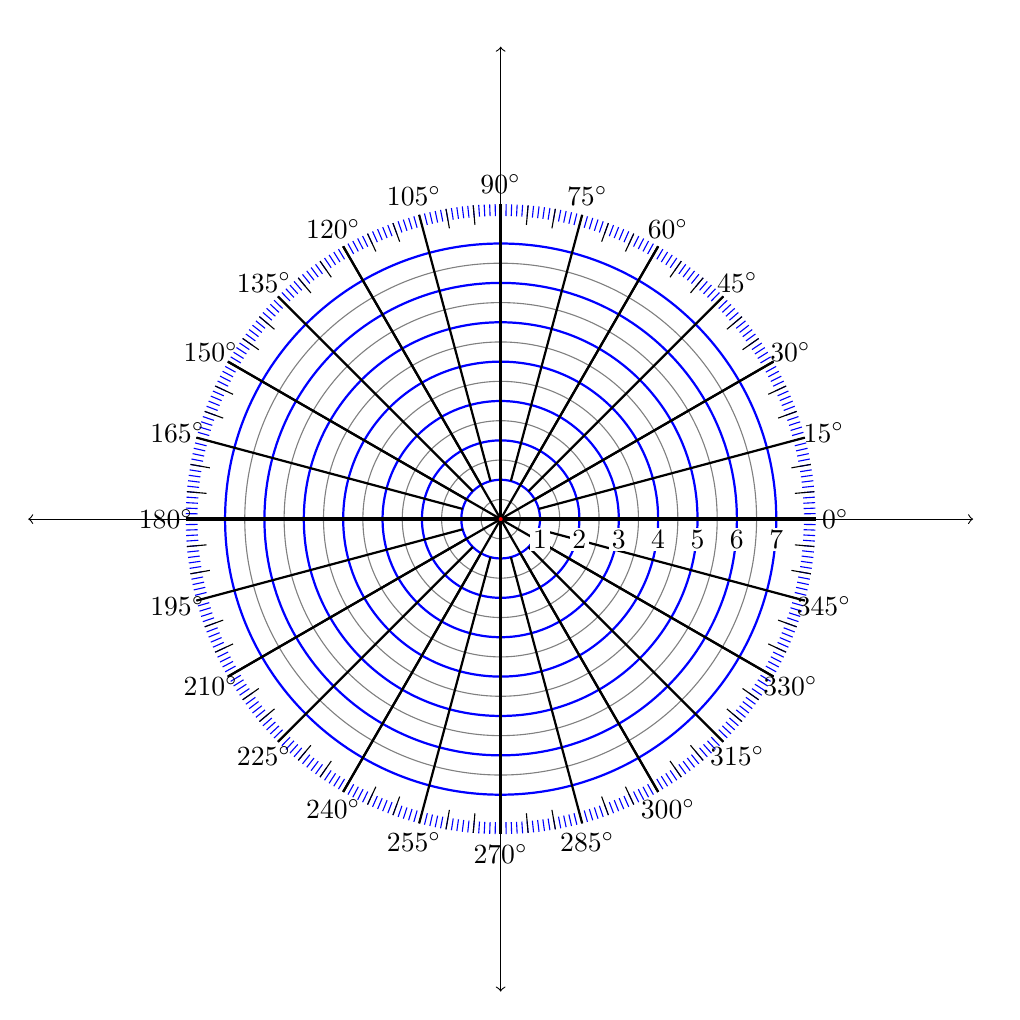
\begin{tikzpicture}[scale = .5]
        \draw[<->] (-12,0)--(12,0) node[right]{$\RE$};
        \draw[<->] (0,-12)--(0,12) node[above]{$\IM$};
    %Circles 
    \foreach \r in {1, 2,...,7}
      \draw[blue, thick] (0,0) circle (\r);    
    \foreach \r in {0.5, 1.5,...,7}
      \draw[gray, thin] (0,0) circle (\r);
    %1° Rays
    \foreach \a in {0, 1,...,359}
      \draw[blue] (\a:7.7) -- (\a:8);
    %5° Rays
    \foreach \a in {0, 5,...,359}
      \draw[black] (\a:7.5) -- (\a:8);      
    %15° Rays
    \foreach \a in {0, 15,...,359}
      \draw[thick,black] (\a:1) -- (\a:8); 
    %30° Rays
    \foreach \a in {0, 30,...,359}
      \draw[thick,black] (0, 0) -- (\a:8);
    %Radius labels (background filled white)
    \foreach \r in {1, 2,...,7}
      \draw (\r,0) node[inner sep=1pt,below=3pt,rectangle,fill=white] {$\r$};
    %Main rays
    \foreach \a in {0, 90,...,359}
      \draw[very thick] (0, 0) -- (\a:8);
    %Angle labels  
    \foreach \a in {0, 15,...,359}
      \draw (\a: 8.5) node {$\a^\circ$};
    %Central point
    \draw[fill=red] (0,0) circle(0.7mm);
  \end{tikzpicture}
\end{center}
In this picture you can see that coordinates are given by a distance from the origin and an angle.  Of course, we remember that we tend to prefer radians, so in this case we would have
\[
0^\circ = 0 \quad 45^\circ = \frac{\pi}{4} \quad 90^\circ = \frac{\pi}{2} \quad 180^\circ = \pi.
\]

\begin{question}
        Do you know where radians come from? Why are they a natural choice for angle?
\end{question}

\begin{answer}
    If we consider the unit circle (a circle with radius one), then its circumference is $2\pi$. Thus, the ``angle" around the unit circle you travel can just be given by the amount of the circumference you have traveled around.
\end{answer}

\begin{exercise}
Identify all the degrees on the above figure with their values in radians.
\end{exercise}

\begin{question}
        If we are given a point in cartesian coordinates (specifying a $\RE$ and $\IM$ part in $\C$ (or $(x,y)$ in $\R^2$), how can we find the polar coordinates $(r, \theta)$? How about vice-versa?
\end{question}
        
        \begin{answer}
            Coming to you now!
        \end{answer}
        
        \subsection{Euler's Formula}
        
        \subsubsection{Taylor Series*}
        This is a brief interlude on something we will get to later in this class.  \emph{Taylor series} are necessary for the \emph{Euler's formula}. Right now I'm just writing it so that I avoid lying to you! Fundamentally, functions we care about can be approximated by their derivatives at a single point. For example, take the function $e^x$.  It turns out, we can write this function in a new way.  That is in the form of a \emph{power series}. In fact, we have 
        \[
        e^x = \sum_{n=0}^\infty \frac{x^n}{n!}.
        \]
        More generally, for other functions (with some sufficient conditions I don't care to get into) we can write:
        \[
        f(x)=\sum_{n=0}^\infty \frac{f^{(n)}(c)}{n!}(x-c)^n.
        \]
        The latter is known as the \emph{Taylor series for $f$ centered at $x=c$}. You really may wonder why in the world I've just introduced this rather abstract concept, but it plays a fundamental role in the complex world.
        
        Using the above Taylor series for $e^x$, we can plug in the following:
        \[
        e^{i\theta}=\sum_{n=0}^\infty \frac{(i\theta)^n}{n!}.
        \]
        It turns out that we find
        \[
        e^{i\theta} = \cos \theta + i \sin \theta.
        \]
        This result is known as \boldgreen{Euler's formula}\index{Euler's formula}. We will do the rest of the work later! Just believe me for now.
        
        It turns out that Euler's formula gives us all the necessary tools to represent numbers in the complex plane in a cartesian or polar way.  So let's do a bit of work to reach this conclusion.
        
        \begin{df}{Modulus}{modulus}
        Given a complex number $z$, the \boldgreen{modulus}\index{modulus} $|z|$ (think \emph{length}) of a complex number is given by
        \[
        |z|=\sqrt{zz^*}.
        \]
        Letting $z=a+bi$ we find
        \[
        |z|=\sqrt{a^2+b^2},
        \]
        which is not entirely shocking.  Just like the lengths of vectors in the plane, the ``length" of a complex number follows suit.
        \end{df}
        
        \begin{question}
                Given any $\theta$, what is the modulus of $z=e^{i\theta}$?
        \end{question}
        
        \begin{answer}
        We take
        \[
        z=e^{i\theta}=\cos \theta + i \sin \theta.
        \]
        Then
        \[
        zz^*=\cos^2 \theta + \sin^2 \theta = 1.
        \]
        So
        \[
        |z|=\sqrt{1}=1.
        \]
        \end{answer}
        
        It turns out that there is a fundamental relationship underlying the complex numbers.  The moral of the story is that imaginary parts of complex numbers cause rotations while the real parts cause scaling. This isn't entirely the case, but it's an alright analogy. We'll be able to uncover this as we explore polar coordinates in more depth.
        
        \begin{remark}
        Something should be said here about the idea of coordinates in general.  Points in a plane are just that -- points.  Where they are located relative to each other is the fundamental structure whereas how we choose to measure this distance is not.  
        
        Polar coordinates are just another way of specifying where a point is located.  This choice of coordinates should not change the behavior of the algebra we have developed or any of the geometry.  Does choosing to measure an object in inches versus centimeters change the length of the object? Of course not.
        \end{remark}
        
        \subsection{Polar Coordinates and Transformations}
        The fact that we can write
        \[
        e^{i\theta}= \cos \theta + i \sin \theta
        \]
        means that we can control the angle of a line that the complex number lives on.  Since the above function lies on the unit circle in $\C$, we can scale this with a real number to reach any point in $\C$. This motivates the following.
        
        \begin{df}{Polar Coordinates}{pol_coord}
        An equivalent way to represent a point in $\C$ is to specify its \boldgreen{argument}\index{argument} (angle, denoted $\arg(z)$) $\theta$ and its \boldgreen{modulus}\index{modulus} (distance from the origin, denoted $r$ or $|z|$) $r$ and write
        \[
        z=re^{i\theta}.
        \]
        We call this coordinate representation \boldgreen{polar coordinates}. 
        \end{df}
        
        Before, we had always written this in a cartesian way, like
        \[
        z=a+bi.
        \]
        But we also have Euler's formula, which means that
        \[
        a+bi = re^{i\theta} = r\cos \theta + i r \sin \theta.
        \]
        This means that
        \[
        a=r\cos \theta
        \]
        and 
        \[
        b = r \sin \theta.
        \]
        You can also see that this is really nothing more than the Pythagorean theorem.
        
        \begin{exercise}
            Pick a point $z$ in the complex plane. Construct a right triangle where the hypotenuse goes from $0$ to $z$ and the other two sides run parallel to the $\RE$ and $\IM$ axes. Can you find $r$ and $\theta$ from this drawing? (\emph{Hint: you will need to use facts from the trigonometry section in the introduction.})
        \end{exercise}
        
        
        
        \noindent \textbf{\textbf{Conversion from polar to cartesian:}} If you're given a point in $\C$ in polar coordinates,
        \[
        z=re^{i\theta},
        \]
        then in cartesian coordinates it will read
        \[
        z=r\cos \theta + ir\sin \theta.
        \]
        This is
        \[
        a=r\cos \theta \qquad b=r\sin \theta.
        \]
        
        \noindent \textbf{\textbf{Conversion from cartesian to polar:}} If you're given a point in $\C$ is cartesian coordinates,
        \[
        z=a+bi,
        \]
        then in polar coordinates it will read
        \[
        z=|z|e^{i\arctan(b/a)},
        \]
        when we have $a>0$. When we have $a<0$ then we have
        \[
        z=-|z|e^{i\arctan(b/a)}=\|z\|e^{i(\arctan(b/a)+\pi)}.
        \]
        That is that the modulus and argument follow
        \[
        r = |z|=\sqrt{zz^*} \qquad \theta = \arctan\left( \frac{b}{a}\right)
        \]
        when $a>0$ and again we have
        \[
        \theta = \arctan\left(\frac{b}{a}\right)+\pi
        \]
        when $a<0$. We defined $|z|$ to be the distance $z$ is from the origin, so this is clear.  The $\arctan(b/a)$ can be realized from the trigonometric fact that
        \[
        \tan \theta = \frac{b}{a}
        \]
        and inverting. If we have that $a=0$, then $\theta=\frac{\pi}{2}$ or $\theta=\frac{3\pi}{2}$. Since we have
        \[
        e^{i\frac{\pi}{2}}=i \qquad \textrm{and} \qquad e^{i\frac{3\pi}{2}}=-i,
        \]
        we need only look at the sign of $b$.  If $b>0$ then $\theta=\frac{\pi}{2}$ and if $b<0$ then $\theta=\frac{3\pi}{2}$.
        
        
        \subsection{Multiplication of complex numbers in polar form}
        
        While we were perfectly happy to multiply complex numbers in Cartesian form, it is more illuminating to multiply them in polar form.  Let us take two complex numbers
        \[
        z_1 = r_1 e^{i\theta_1} \qquad z_2 = r_2 e^{i\theta_2}.
        \]
        Then we can write the product:
        \[
        z=z_1 z_2 = (r_1 e^{i\theta_1})(r_2 e^{i\theta_2})= r_1r_2 e^{i(\theta_1+\theta_2)}.
        \]
        The thing to notice here is that the modulus of a product follows
        \[
        |z|=|z_1||z_2|=r_1r_2
        \]
        and the argument of a product follows
        \[
        \arg(z)=\arg(z_1)+\arg(z_2).
        \]
        All of this is to say to the following: Multiplication of complex numbers is decomposed into rotation and scaling. 
        
        \begin{center}
            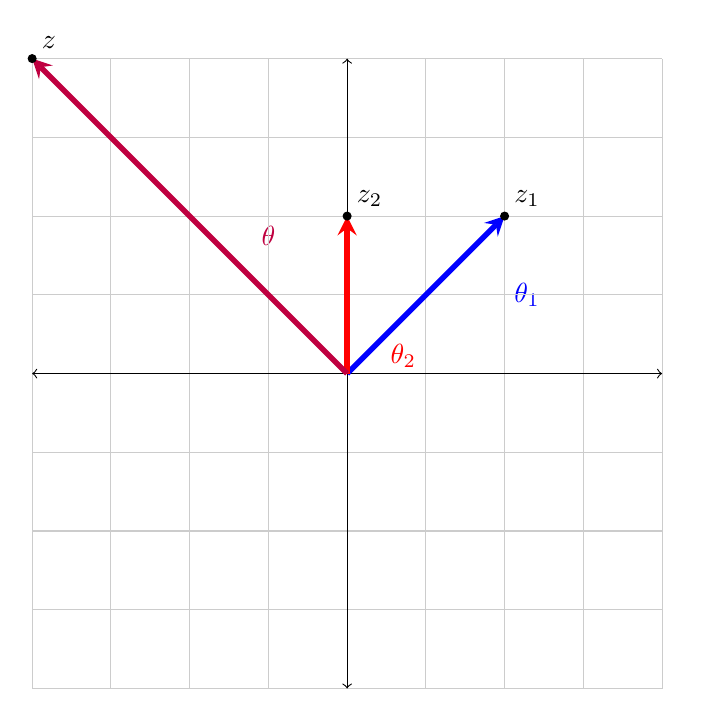
\begin{tikzpicture}
            \tdplotdrawarc[->,line width = 1pt, blue]{(0,0)}{2}{0}{45}{}{};
            \node[anchor=west] at (2,1){$\color{blue}{\theta_1}$};
            \tdplotdrawarc[->,line width = 1pt, red]{(0,0)}{1}{0}{90}{}{};
            \node[anchor=north east] at (1,.5){$\color{red}{\theta_2}$};
            \tdplotdrawarc[->,line width = 1pt, purple]{(0,0)}{1.5}{0}{135}{}{};
            \node[anchor=north] at (-1,2){$\color{purple}{\theta}$};
            \draw[thin,gray!40] (-4,-4) grid (4,4);
            \draw[<->] (-4,0)--(4,0) node[right]{$\RE$};
            \draw[<->] (0,-4)--(0,4) node[above]{$\IM$};
            \draw[line width=2pt,blue,-stealth](0,0)--(2,2) node[anchor=east] at (1,1){};
            \draw[line width=2pt,red,-stealth](0,0)--(0,2) node[anchor=east] at (2,-1){};
            \draw[line width=2pt,purple,-stealth](0,0)--(-4,4) node[anchor=east] at (2,-1){};
            \foreach \Point/\PointLabel in {(-4,4)/z, (2,2)/z_1, (0,2)/z_2}
            \draw[fill=black] \Point circle (0.05) node[above right] {$\PointLabel$};
            \end{tikzpicture}
        \end{center}
    
    
        \subsubsection{Inverse in polar form}
        We found before that given a complex number $z$, we can find the inverse $z^{-1}=1/z$ in cartesian form.  But this was a bit of a headache.  In polar form, however, it is much easier.  Recall that if we have
        \[
        z_1 z_2 = \left(r_1e^{i\theta_1}\right)\left(r_2e^{i\theta_2}\right)=r_1r_2e^{i(\theta_1+\theta_2)}.
        \]
        
        Now, given $z=re^{i\theta}$ we can find fairly quickly that $z^{-1}$ must be
        \[
        z^{-1}=\frac{1}{r}e^{-i\theta}.
        \]
        
        \begin{exercise}
        Show that this is indeed the inverse. (\emph{Hint: take our example $z^{-1}$ and multiply it by $z=re^{i\theta}$ and see that you get one.})
        \end{exercise}
        
        \section{Periodic Motion}
        
        One of the greatest benefits to complex numbers is the ability to naturally capture rotations.  When we wrote complex numbers in polar form, the rotation action became more clear. This ability makes complex numbers very useful in systems that rotate, oscillate, or have some kind of \emph{periodic} motion.
        
        \begin{question}
                What is periodic motion?
        \end{question}
        
        \begin{answer}
            Periodic motion is when a system undergoes a change that repeats itself.  For example, a mass attached to a spring will vibrate back and forth.  As the mass moves from one side to the other, it eventually gets back to where it started and repeats the process again (with no friction, of course).
        \end{answer}
        
        \noindent There is a great example of periodic motion in the complex numbers that we should take a look at.  
        
        \begin{ex}{Circular Motion}{circ_motion}
            Let us consider the function $f\colon \R \to \C$ given by
            \[
            f(t)=e^{it}.
            \]
            What happens as $t$ increases? Let's let $0<t_1<t_2<t_3<t_4<2\pi$ for now and we can plot this
            \begin{center}
            \begin{tikzpicture}
            \tdplotdrawarc[->,line width = 1pt, black]{(0,0)}{3}{0}{45}{}{};
            \node[anchor=west] at (2.75,1.25){${t_1}$};
            \tdplotdrawarc[->,line width = 1pt, black]{(0,0)}{2.25}{0}{90}{}{};
            \node[anchor=north east] at (1.5,2.5){${t_2}$};
            \tdplotdrawarc[->,line width = 1pt, black]{(0,0)}{1.5}{0}{180}{}{};
            \node[anchor=south east] at (-1,1){${t_3}$};
            \tdplotdrawarc[->,line width = 1pt, black]{(0,0)}{1}{0}{270}{}{};
            \node[anchor=north east] at (-.6,-.6){${t_4}$};
            \draw[<->] (-5,0)--(5,0) node[right]{$\RE$};
            \draw[<->] (0,-5)--(0,5) node[above]{$\IM$};
            \draw[line width=2pt,black,-stealth](0,0)--(0,4) node[anchor=south east] at (0,4){$f(t_2)$};
            \draw[line width=2pt,black,-stealth](0,0)--(2.828,2.828) node[anchor=south east] at (2.828,2.828){$f(t_1)$};
            \draw[line width=2pt,black,-stealth](0,0)--(-4,0) node[anchor=south] at (-4,0){$f(t_3)$};
            \draw[line width=2pt,black,-stealth](0,0)--(0,-4) node[anchor=east] at (0,-4){$f(t_4)$};
            % \foreach \Point/\PointLabel in {(-4,4)/z, (2,2)/z_1, (0,2)/z_2}
            % \draw[fill=black] \Point circle (0.05) node[above right] {$\PointLabel$};
            \end{tikzpicture}
        \end{center}
        Notice that by choosing $t$ in this way we have that $t$ corresponds to the angle of rotation $\theta$. 
        \end{ex}
        
        \begin{question}
            What happens when we let $t>2\pi$? 
        \end{question}
        
        \begin{answer}
            We come back around the circle. For example, if we take $\theta=\frac{\pi}{4}$ and $\Theta=2\pi + \frac{\pi}{4}$ and plug these values in to $e^{it}$ then we find:
            \begin{center}
            \begin{tikzpicture}
            \tdplotdrawarc[->,line width = 1pt, black]{(0,0)}{2}{45}{405}{}{};
            \node[anchor=west] at (0,2.25){$2\pi$};
            \tdplotdrawarc[->,line width = 1pt, black]{(0,0)}{3}{0}{45}{}{};
            \node[anchor=west] at (2.75,1.25){$\theta$};
            \draw[<->] (-3,0)--(5,0) node[right]{$\RE$};
            \draw[<->] (0,-3)--(0,5) node[above]{$\IM$};
            \draw[line width=2pt,black,-stealth](0,0)--(2.828,2.828) node[anchor=south east] at (2.828,2.828){${e^{i\theta}=e^{i\Theta}}$};
            % \foreach \Point/\PointLabel in {(-4,4)/z, (2,2)/z_1, (0,2)/z_2}
            % \draw[fill=black] \Point circle (0.05) node[above right] {$\PointLabel$};
            \end{tikzpicture}
        \end{center}
        We can see that if we add $2\pi$ to any angle $\theta$ we get back to the original angle.  
        \end{answer}
        
        \begin{df}{Periodic Function}{periodic_func}
            A function $f$ with real inputs is \boldgreen{periodic}\index{periodic} with period $T$ if 
            \[
            f(x)=f(x+T)
            \]
            for all $x$.
        \end{df}
        
        \begin{exercise}
        Realize the function $f\colon \R \to \C$ given by
        \[
        f(t)=e^{it}
        \]
        as periodic with period $2\pi$.
        \end{exercise}
        
        \begin{exercise}
        Can you name two more periodic functions with period $2\pi$? 
        \end{exercise}
        
        \begin{exercise}
        Show that the function 
        \[
        g(t)=e^{i\frac{2\pi t}{T}}
        \]
        is periodic with period $T$.
        \end{exercise}
        
        \begin{df}{Frequency}{freq}
        Let $f$ be a periodic function with period $T$. Then its \boldgreen{frequency}\index{frequency} is
        \[
        \nu = \frac{1}{T}.
        \]
        \end{df}
        
        \newpage
        
        \section{Problems}
        
        \begin{problem}
        Complete the exercises throughout the chapter.
        \end{problem}
        
        \begin{problem}
        ... To come.
        \end{problem}